\documentclass[12pt, twoside]{article}
\usepackage[letterpaper, margin=1in, headsep=0.2in]{geometry}
\setlength{\headheight}{0.6in}
%\usepackage[english]{babel}
\usepackage[utf8]{inputenc}
\usepackage{microtype}
\usepackage{amsmath}
\usepackage{amssymb}
%\usepackage{amsfonts}
\usepackage{siunitx} %units in math. eg 20\milli\meter
\usepackage{yhmath} % for arcs, overparenth command
\usepackage{tikz} %graphics
\usetikzlibrary{quotes, angles}
\usepackage{graphicx} %consider setting \graphicspath{{images/}}
\usepackage{parskip} %no paragraph indent
\usepackage{enumitem}
\usepackage{multicol}
\usepackage{venndiagram}

\usepackage{fancyhdr}
\pagestyle{fancy}
\fancyhf{}
\renewcommand{\headrulewidth}{0pt} % disable the underline of the header
\raggedbottom
\hfuzz=2mm %suppresses overfull box warnings

\usepackage{hyperref}

\fancyhead[LE]{\thepage}
\fancyhead[RO]{\thepage \\ Name: \hspace{4cm} \,\\}
\fancyhead[LO]{BECA / Dr. Huson / Geometry\\*  Unit 4: Volume and polyhedra \\* 2 November 2022}

\begin{document}

\subsubsection*{4.3 Homework: Angle review}
\begin{enumerate}
\item Given $\overline{JKL}$, $JK=5.4$, and $KL=1.1$. Find ${JL}$.\\[0.5cm]
Show your work by marking the diagram and writing an equation.\\[2cm]
  \begin{tikzpicture}
    \draw [-, thick] (0,0)--(7,0);
    \draw [fill] (0,0) circle [radius=0.05] node[below]{$J$};
    \draw [fill] (5,0) circle [radius=0.05] node[below]{$K$};
    \draw [fill] (7,0) circle [radius=0.05] node[below]{$L$};
  \end{tikzpicture}

\item A parallelogram is shown on the $x$-$y$ plane having a base $b=2.5$ and height $h=4.0$. 
  \begin{multicols}{2}
    Find its area, showing the calculation.
      \begin{flushright}
      \begin{tikzpicture}[scale=.635]
        %\draw [help lines] (-1,-1) grid (9,6);
        \draw [thick, ->] (-1.2,0) -- (7.4,0) node [below right] {$x$};
        \draw [thick, ->] (0,-1.2)--(0,6.4) node [left] {$y$};
        \draw [<->, thick] (1.5,1)--(1.5,5);
        \draw [-, thick] (2,1)--(4.75,1)--(5.75,5)--(3,5)--cycle;
        \node at (3.5,1)[below]{$2.5$};
        \node at (1.5,3)[left]{$4.0$};
      \end{tikzpicture}
      \end{flushright}
  \end{multicols} 

\item Subtract to find the length between $P(-3)$ and $Q(2)$. Take the absolute value if necessary since lengths are positive numbers. \\[0.25cm]
  \begin{tikzpicture}
    \draw [<->] (-4.5,0)--(4.5,0);
    \draw [-, thick] (-3,0)--(2,0);
    \foreach \x in {-4,...,4} %2 leading for diff!=1
      \draw[shift={(\x,0)},color=black] (0pt,-3pt) -- (0pt,3pt) node[below=5pt]  {$\x$};
      \draw [fill] (-3,0) circle [radius=0.05] node[above] {$P$};
      \draw [fill] (2,0) circle [radius=0.05] node[above] {$Q$};
  \end{tikzpicture}

\item As shown below, two lines intersect making four angles: $\angle 1$, $\angle 2$, $\angle 3$, and $\angle 4$.
  \begin{multicols}{2}
    Given $m\angle 2 = 105^\circ$.  
    \begin{enumerate}
      \item Find $m\angle 3$ \vspace{2cm}
      \item Find $m\angle 4$ \vspace{2cm}
    \end{enumerate}
    \begin{tikzpicture}[scale=0.7, rotate=20]
    \draw [<->, thick] (0,-1.5)--(10,1.5);
    \draw [<->, thick] (2,3.5)--(7,-3.5);
    \node at (3,.4){1};
    \node at (6,-.6){3};
    \node at (5,1){2};
    \node at (4,-1){4};
  \end{tikzpicture}
  \end{multicols}

\newpage
\item Given $\overline{ABC}$, $AB=2x+2$, $BC=6$, $AC=14$. Find ${x}$.
\begin{center}
    \begin{tikzpicture}
    \draw [-, thick] (0,0)--(7,0);
    \draw [fill] (0,0) circle [radius=0.05] node[below]{$A$};
    \draw [fill] (4,0) circle [radius=0.05] node[below]{$B$};
    \draw [fill] (7,0) circle [radius=0.05] node[below]{$C$};
    \node at (2,0) [above]{$2x+2$};
    \node at (5.5,0) [above]{$6$};
    \draw [<->, dashed] (0,-0.7)--(7,-0.7);
    \node at (3.5,-0.7) [below]{$14$};
  \end{tikzpicture}
\end{center} \vspace{3cm}

\item Find the volume of a rectangular prism (box). Its length is $l=19$ inches, its height $h=11$ inches, and depth is $w=7$ inches. Start with the equation \\[0.5cm]
$V = l \times w \times h$
  \begin{flushright}
    \begin{tikzpicture}[scale=1.25]
      \draw [-, thick] (0,0)--(4,0)--(4,2)--(0,2)--cycle;
      \draw [-, thick] (0,2)--(0.5,2.75)--(4.5,2.75)--(4,2);
      \draw [-, thick] (4,0)--(4.5,0.75)--(4.5,2.75);
      \node at (4.75, 1.75){$11$};
      \node at (2, -0.25){$19$};
      \node at (4.5, 0.25){$7$};
    \end{tikzpicture}
  \end{flushright}


\item Apply the Angle Addition postulate. Write and equation to support your work.
  \begin{multicols}{2}
    Given $m\angle CBD = 28^\circ$, $m\angle ABC = 90^\circ$. \\[0.5cm]
    Find $m \angle ABD$. \\
    \begin{tikzpicture}[scale=1.4]
      \draw [<->, thick]
        (0:3) coordinate (a) node[below left] {$C$}
        -- (0,0) coordinate (b) node[below left] {$B$}
        -- (30:3) coordinate (c) node[below right] {$D$}
        pic["$28^\circ$", <->, draw=black, angle eccentricity=1.5, angle radius=1cm]
        {angle=a--b--c};
        \draw [<-, thick]
        (90:2) coordinate (d) node[right] {$A$}
        -- (0,0) coordinate (e)
        pic["$?$", <->, draw=black, angle eccentricity=1.25, angle radius=1cm]
        {angle=c--e--d};
      \draw (0,0)++(0.3,0)--++(0,0.3)--+(-0.3,0);
    \end{tikzpicture}
  \end{multicols}

\newpage
\item Find the length of the base of a rectangle with area $A=64$ and height $h=16$. Start with the form (use $b$ or $x$): \\[0.5cm]
$A = b \times h = 64$
  \begin{flushright}
  \begin{tikzpicture}[scale=1.25]
    \draw [-, thick] (0,0)--(2,0)--(2,5)--(0,5)--cycle;
    \node at (2.5, 2.5){$16$};
    \node at (1, -0.5){$?$};
    \node at (1, 3){$64$};
  \end{tikzpicture}
  \end{flushright}

\item Given $S(-1.4)$ and $T(5.4)$, as shown on the number line. \\[0.25cm]
  Mark and label the midpoint $M$ that bisects $\overline{ST}$. \\[0.5cm]
    \begin{tikzpicture}
      \draw [<->] (-3.5,0)--(6.5,0);
      \draw [-, thick] (-1.4,0)--(5.4,0);
      \foreach \x in {-3,...,6} %2 leading for diff!=1
        \draw[shift={(\x,0)},color=black] (0pt,-3pt) -- (0pt,3pt) node[below=5pt]  {$\x$};
        \draw [fill] (-1.4,0) circle [radius=0.05] node[above] {$S$};
        \draw [fill] (5.4,0) circle [radius=0.05] node[above] {$T$};
    \end{tikzpicture}
    \begin{flushright}
      Write the value of $M$ in the box.
    \end{flushright}
    
\item The perimeter of the isosceles $\triangle FGH$ is $18 \frac{1}{2}$ with $\overline{FH} \cong \overline{GH}$. If $FG=x+2$ and $FH=7 \frac{1}{4}$, find $x$.\\[0.25cm]
  Show your work with an equation.\\[0.5cm]
    \begin{tikzpicture}[scale=0.5]
      \draw [thick](0,0)--(4,0)--(2,6)--(0,0);
      \draw [fill] (0,0) circle [radius=0.05] node[below left]{$F$};
      \draw [fill] (4,0) circle [radius=0.05] node[below right]{$G$};
      \draw [fill] (2,6) circle [radius=0.05] node[above right]{$H$};
      \draw [thick] (0.8,3.1)--(1.2,3); %tick mark
      \draw [thick] (2.8,3)--(3.2,3.1); %tick mark
      \node at (2,0) [below]{$x+2$};
      \node at (0.8,3.4) [left]{$7 \frac{1}{4}$};
    \end{tikzpicture}
    \begin{flushright}
      Write the value of $x$ in the box.
    \end{flushright}

\item A linear pair is formed by two angles, $m\angle RUT = 4x+14$ and $m\angle SUT = 6x-4^\circ$. \\[0.5cm] 
Write an equation, then solve for $x$. \vspace{0.5cm}
  \begin{flushright}
    \begin{tikzpicture}[scale=1]
      \draw [<->, thick]
        (0:5) coordinate (a) node[below left] {$S$}
        -- (0,0) coordinate (b) node[below] {$U$}
        -- (95:3) coordinate (c) node[above right] {$T$}
        pic["$6x-4^\circ$", <->, draw=black, angle eccentricity=1.5, angle radius=1.5cm]
        {angle=a--b--c};
        \draw [<-, thick]
        (180:4) coordinate (d) node[below] {$R$}
        -- (0,0) coordinate (e)
        pic["$4x+14$", <->, draw=black, angle eccentricity=1.5, angle radius=1.5cm]
        {angle=c--e--d};
    \end{tikzpicture}
  \end{flushright}

\item The rectangular prism shown has a volume of $V=615$ cubic feet. Its base measures $l=8.2$ feet by $w=6.25$ feet. \\[0.5cm]
Find its height. Begin by writing the following formula with values substituted: \\[0.5cm]
$V = l \times w \times h = 615$
\begin{flushright}
  \begin{tikzpicture}[scale=1]
    \draw [-, thick] (0,0)--(3,0)--(3,4)--(0,4)--cycle;
    \draw [-, thick] (0,4)--(0.5,4.75)--(3.5,4.75)--(3,4);
    \draw [-, thick] (3,0)--(3.5,0.75)--(3.5,4.75);
    \node at (3.75, 2.75){$h$};
    \node at (1.5, -0.25){$8.2$};
    \node at (4, 0.25){$6.25$};
  \end{tikzpicture}
\end{flushright}

\item Find the area of circle $Q$ with radius $r=5.0$ centimeters, rounded to the \emph{nearest tenth}.
  Start with the formula\\[0.5cm]
  $A = \pi r^2$ 
    \begin{flushright}
      \begin{tikzpicture}[scale=1]
        \draw (0,0) circle[radius=3];
        \draw [thick]
        (0:3) node[right] {$P$}--
        (0,0) node[below] {$Q$};
        \draw (1.5,0) node[below] {$5.0$};
      \end{tikzpicture}
    \end{flushright}

\item In the diagram shown, $\overrightarrow{BD} \perp \overleftrightarrow{ABC}$ and angle measures are given. \\[0.5cm] 
Find $x$.\vspace{0.5cm}
  \begin{multicols}{2}
    $m\angle DBE = 5x+21^\circ$ \\[0.25cm]
    $m\angle EBC = 19x-27^\circ$ \\[0.25cm]
    \begin{tikzpicture}[scale=1]
      \draw [<->, thick]
        (0:5) coordinate (a) node[below left] {$C$}
        -- (0,0) coordinate (b) node[below] {$B$}
        -- (50:5) coordinate (c) node[below right] {$E$}
        pic["$19x-27$", <->, draw=black, angle eccentricity=1.5, angle radius=1.5cm]
        {angle=a--b--c};
        \draw [<-, thick]
        (90:4) coordinate (d) node[right] {$D$}
        -- (0,0) coordinate (e)
        pic["$5x+21$", <->, draw=black, angle eccentricity=1.5, angle radius=1.5cm]
        {angle=c--e--d};
        \draw [->, thick] (0,0)--(-180:2) node[below right]{$A$};
        \draw (0,0)++(-0.3,0)--++(0,0.3)--+(0.3,0);
    \end{tikzpicture}
  \end{multicols}

\item Find the length of the base of a triangle with area $A=35.7$ and height $h=8.5$. Express your result as a decimal. Start with the form (use $b$ or $x$): \\[0.5cm]
$A = \frac{1}{2} \times b \times h = 35.7$
  \begin{flushright}
  \begin{tikzpicture}[scale=1.25]
    \draw [-, thick] (-1,0)--(3,0)--(2.5,3.5)--cycle;
    \node at (3.3, 1.5){$8.5$};
    \node at (1, -0.5){$?$};
    \node at (1.5, 1){$A = 35.7$};
  \end{tikzpicture}
  \end{flushright}

\item Given $\overleftrightarrow{ABC}$, right angle $\angle DBE$, $m\angle ABE = 6x+8$, and $m\angle DBC = 4x-3$. \\[0.5cm] 
Find $x$. \vspace{0.5cm}
  \begin{flushright}
    \begin{tikzpicture}[scale=1, rotate=30]
      \draw [<->, thick]
        (-30:5) coordinate (a) node[below left] {$C$}
        -- (0,0) coordinate (b) node[below] {$B$}
        -- (3,0) coordinate (c) node[below right] {$D$}
        pic["$4x-3$", <->, draw=black, angle eccentricity=1.5, angle radius=1.5cm]
        {angle=a--b--c};
        \draw [<->, thick]
        (150:4) coordinate (d) node[below] {$A$}
        -- (0,0) -- (0, 3) coordinate (e) node[right] {$E$}
        pic["$6x+8$", <->, draw=black, angle eccentricity=1.5, angle radius=1.5cm]
        {angle=e--b--d};
        \draw (0,0)++(0.4,0)--++(0,0.4)--+(-0.4,0);
    \end{tikzpicture}
  \end{flushright}
  \begin{flushright}
    Write the value of $x$ as a decimal.
  \end{flushright}

\item Given $\overline{PQR}$, $PQ=3x+13$, $QR=2x-1$, $PR=x+28$. Find ${x}$.
  \begin{center}
      \begin{tikzpicture}
      \draw [-, thick] (0,0)--(7,0);
      \draw [fill] (0,0) circle [radius=0.05] node[below]{$P$};
      \draw [fill] (5,0) circle [radius=0.05] node[below]{$Q$};
      \draw [fill] (7,0) circle [radius=0.05] node[below]{$R$};
      \node at (2,0) [above]{$3x+13$};
      \node at (6,0) [above]{$2x-1$};
      \draw [<->, dashed] (0,-0.7)--(7,-0.7);
      \node at (3.5,-0.7) [below]{$x+28$};
    \end{tikzpicture}
  \end{center}

\item Ray $\overrightarrow{BF}$ is the angle bisector of $\angle ABC$. Given that the angle measures are $m\angle ABF = 8x-14$ and $m\angle CBF = 6x+8$. \\[0.5cm] 
Find $x$. \vspace{0.5cm}
  \begin{flushright}
    \begin{tikzpicture}[scale=1]
      \draw [<->, thick]
        (0:5) coordinate (a) node[below left] {$C$}
        -- (0,0) coordinate (b) node[below] {$B$}
        -- (70:3) coordinate (c) node[above right] {$F$}
        pic["$6x+8$", <->, draw=black, angle eccentricity=1.75, angle radius=1.5cm]
        {angle=a--b--c};
        \draw [<-, thick]
        (140:4) coordinate (d) node[below] {$A$}
        -- (0,0) coordinate (e)
        pic["$8x-14$", <->, draw=black, angle eccentricity=1.25, angle radius=1.5cm]
        {angle=c--e--d};
        %\draw [->, thick] (0,0)--(-180:2) node[below right]{$A$};
        %\draw (0,0)++(-0.3,0)--++(0,0.3)--+(0.3,0);
    \end{tikzpicture}
  \end{flushright}
  

\end{enumerate}
\end{document}